\documentclass[10pt,xcolor={table,dvipsnames}]{beamer} 		% carica automaticamente amsthm, amssymb, amsmath, graphicx
\setbeamertemplate{theorems}[numbered]%[ams style] 


\usepackage[T1]{fontenc}				% codifica dei font
\usepackage[utf8]{inputenc}				% lettere accentate da tastiera
\usepackage[italian]{babel}				% lingua del documento
\usepackage[italian]{varioref}			% Per usare il comando \vref{label}, che dà dei collegamenti più dettagliati

% Load the custom style file
\usepackage{AndreaStyle}
% The file `AndreaStyle.sty` is stored in: `D:\Programmi e Applicazioni\texlive\texmf-local\tex\latex\local` for Windows.
% The file `AndreaStyle.sty` is stored in: `/usr/local/texlive/texmf-local/tex/latex/local` for Ubuntu (desktop).
% This won't work in Overleaf, until the AndreaStyle.sty file is added to the project

\usepackage{mathdots}

%\usepackage{algorithm}
%\usepackage[beginLComment=//~,endLComment=~]{algpseudocodex}			% Package for typesetting algorithms

\usepackage{mathrsfs}					% Per dei caratteri matematici migliori: \mathscr{} e \mathcal{}
%\usepackage{braket} 					% Per il comando \Set, e altre (poche) cose
%\usepackage{textcomp}					% Dovrebbe aggiungere più simboli
\usepackage{bbm}						% Più simboli in \mathbb

%\usepackage{arydshln}					% per le linee tratteggiate nelle tabelle

%\usepackage[rightcaption]{sidecap}		% Per mettere le didascalie di lato

\usepackage{fontawesome5}				% Aggiunge simboli da FontAwesome

\usepackage{hyperref}					% Importante: hyperref va caricato nel documento.


%\setcounter{tocdepth}{1}	% profondità dell'indice

	% TEOREMI CUSTOM:
\theoremstyle{plain}					% Definisce ambienti per Teoremi, esercizi, corollari... Con lo stile adeguato
	\newtheorem{proposizione}{Proposizione}%[section]
	\newtheorem*{proposizione*}{Proposizione}
	
	\newtheorem{teorema}{Teorema}%[section]
	\newtheorem*{teorema*}{Teorema}
		
	%\newtheorem{lemma_es}{Lemma}[esercizio]
	%\newtheorem{lemma}{Lemma}[section]
	\newtheorem*{lemma*}{Lemma}
	\newtheorem{corollario}{Corollario}[section]


\theoremstyle{definition}				
	\newtheorem{definizione}{Definizione}%[section]%[chapter]
	\newtheorem*{definizione*}{Definizione}	%definizione non numerata
	\newtheorem*{notazione}{Notazione}

\theoremstyle{remark}
	\newtheorem{oss}{Osservazione}%[section]
	\newtheorem*{oss*}{Osservazione}


	% COMANDI CUSTOM
% Define the \indicator command
\NewDocumentCommand{\indicator}{O{t} O{m} O{i}}{%
  \mathlarger{\mathbbm{1}}\qty{\scriptstyle {x}_{#1}^{#2}=#3}%
}
% Define the \transpose command
\newcommand{\transpose}[1]{\prescript{t}{}{#1}}
% Define the \Var command, for the variance
\newcommand{\Var}[1]{\operatorname{Var}\qty(#1)}
% Define the \Cov command, for the covariance
\newcommand{\Cov}[1]{\operatorname{Cov}\qty(#1)}

% Define a command to create unnumbered footnotes
\let\svthefootnote\thefootnote
\textheight 1in
\newcommand\blankfootnote[1]{%
  \let\thefootnote\relax\footnotetext{#1}%
  \let\thefootnote\svthefootnote%
}
% Define the \independent symbol, for independence
\newcommand\independent{\protect\mathpalette{\protect\independenT}{\perp}}
    \def\independenT#1#2{\mathrel{\rlap{$#1#2$}\mkern2mu{#1#2}}}

%% Rename keywords for algorithms
%\algrenewcommand\algorithmicrequire{\textbf{Input:}}
%\algrenewcommand\algorithmicensure{\textbf{Output:}}





	%COLORI
\definecolor{madridlightblue}{RGB}{233, 233, 243}
	

	
% ------------------------- INIZIO CODICE -------------------------
\usetheme{Madrid}


\title[Seminario MNCM]{Consistently Estimating Markov Chains with Noisy Aggregate Data}			%WIP
%\subtitle{Presentazione e dimostrazione della convergenza} 
\author{Andrea Marino}
\institute[DI UniPi]{Università di Pisa}
%\titlegraphic{\includegraphics[width=2cm]{Immagini/cherubino_black.eps}}
\date[\today]{Metodi Numerici per le Catene di Markov\newline Seminario di fine corso}

%\AtBeginSubsection[] 						
%{
%	\begin{frame}
%		\frametitle{Sommario}
%		\tableofcontents[currentsection,subsectionstyle=show/shaded/hide] 
%	\end{frame}
%}

%% ----------- ALTERNATIVA -----------
% Custom command to insert the summary frame
\newcommand{\insertSummaryFrame}{
    \begin{frame}
        \frametitle{Sommario}
        \tableofcontents[currentsection, subsectionstyle=show/shaded/hide]
    \end{frame}
}

% Show summary at the beginning of each section
\AtBeginSection[]
{
    \begin{frame}
        \frametitle{Sommario}
        \tableofcontents[currentsection, subsectionstyle=show/hide/hide]
    \end{frame}
}

% Show summary at the beginning of each subsection
\AtBeginSubsection[]
{
    \begin{frame}
        \frametitle{Sommario}
        \tableofcontents[currentsection, subsectionstyle=show/shaded/hide]
    \end{frame}
}


\begin{document}
	\begin{frame}[plain]
		\titlepage
	\end{frame}
	
\section*{Sommario}
	\setcounter{tocdepth}{1}
	\begin{frame}
		\frametitle{Sommario}
		\tableofcontents
	\end{frame}
	
	\setcounter{tocdepth}{2}



\section{Introduzione, notazione e prime definizioni}
	\subsection{Descrizione del problema}

	\begin{frame}{Introduzione al problema, notazione, modello 1/2}%{Descrizione del contesto}
		Supponiamo di avere una popolazione di $N\in\mathbb{N}_{>0}$ individui che evolvono da 
		uno stato all'altro {\smaller ($S\in\mathbb{N}_{>0}$: numero di possibili stati)}, 
		\emph{indipendentemente}, per $T\in\mathbb{N}_{>0}$ istanti temporali 
		{\smaller ($[k]\coloneqq\qty{1,\dots,k}$)}:
		\[
			\qty{x_{t}^{(m)}}_{t\in[T]}\sim\mathrm{Markov}\qty(\pi_0,P)\qquad\forall\,m\in[N].
		\]
		%\vspace*{-\baselineskip}
		%\begin{itemize}
		%	%\item<2-> $N$: dimensione della popolazione, $T$: istanti temporali {\smaller(sarà $T\to\infty$)}
		%	\item<2-> $S\in\mathbb{N}_{>0}$: numero di possibili stati
		%	\item<3-> $P\in\R{S}{S}$: matrice di transizione, $\pi_0\in\R{S}$: distribuzione iniziale
		%\end{itemize}
		%\onslide<2->{$S\in\mathbb{N}_{>0}$: numero di possibili stati, 
		%$P\in\R{S}{S}$: matrice di transizione, 
		%$\pi_0\in\R{S}$: distribuzione iniziale,
		%$\pi\in\R{S}$: distribuzione invariante.}
		%\smallskip 
		
		\onslide<2->{Supponiamo inoltre che:}
		\begin{itemize}
			\item<2-> La catena sia \emph{ergodica} e omogenea nel tempo
			(cfr. Appendice~\hyperlink{frame:catena_ergodica:appendice}{\faHandPointRight}).

			$\pi\in\R{S}$: distribuzione invariante 
			\item<3-> $x_t^{(m)}$ non sia osservabile per alcun $t\in[T], m\in[N]$, 
			ma che vi sia una \emph{conta aggregata} $\vb*{n}_t\in\R{S}$, definita t.c.
			\vspace*{-0.5\baselineskip}
			\[
				\vb*{n}_t(i)\coloneqq\sum_{m=1}^N\indicator
			\]
			\vspace*{-0.9\baselineskip}
			%$\vb*{n}_t(i)\coloneqq\sum_{m=1}^N\indicator$
			\item<4-> I dati osservati siano $\qty{\vb*{y}_1,\dots,\vb*{y}_T}$, 
			$\vb*{y}_t$ è ottenuto 
			da $\vb*{n}_t$ tramite un modello del rumore $\P{\vb*{y}_t}{\vb*{n}_t}$
			\item<5-> La raccolta è ripetuta $K$ volte, restituendo 
			$\qty{\vb*{y}_1^{(k)},\dots,\vb*{y}_T^{(k)}}_{k\in[K]}$
		\end{itemize}
	\end{frame}

	\begin{frame}{Introduzione al problema, notazione, modello 2/2}
		\begin{figure}[ht]
			\centering
			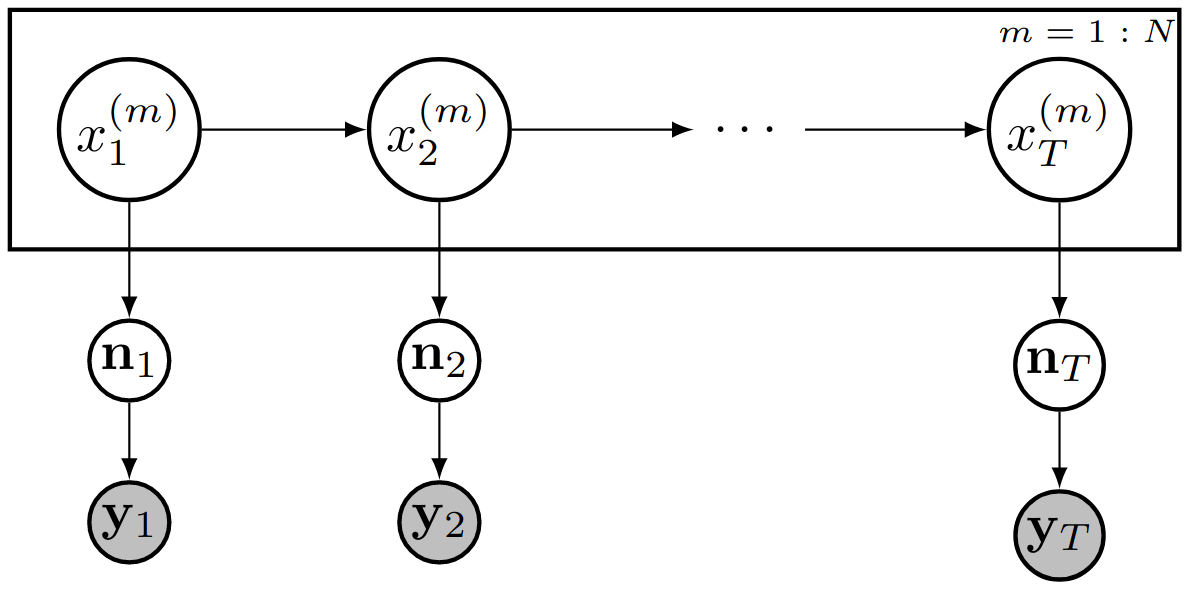
\includegraphics[width=0.45\textwidth]{Immagini/plate_model.png}
			\caption{\emph{Rappresentazione del modello in plate notation}}
		\end{figure}

		\vspace*{-0.5\baselineskip}
		La plate notation rappresenta graficamente come fattorizzare la legge congiunta:
		\begin{itemize}
			\item Cerchio vuoto: v.a. non osservata. Cerchio pieno: v.a. osservata
			\item<2-> Freccia: la v.a. in coda d'arco "influenza" la v.a. in testa
			\item<3-> Rettangolo: copia il contenuto tante volte quanto specificato dall'indice
		\end{itemize}

		%RIMANEGGIARE
		\begin{alertblock}<4->{Obiettivo}
			Usando le osservazioni
			$\big\{\vb*{y}_1^{(k)},\dots,\vb*{y}_T^{(k)}\big\}_{k\in [K]}$, stimare $P$.

			In particolare, vedremo come stimare $P$ usando il \emph{metodo dei momenti}.
			Lo stimatore dei momenti è consistente. 
		\end{alertblock}

	\end{frame}


	\subsection{Osservazioni su \texorpdfstring{$\vb*{n}_t$}{n_t} e su \texorpdfstring{$P$}{P}}

	\begin{frame}
		{\hypertarget{frame:dettagli_nt}{Osservazioni su $\vb*{n}_t$ e su $P$}}
		\begin{definizione*}
			Siano $\vb*{\mu}_t\in\R{S}$ e $\vb*{\mu}_{t,t+1}\in\R{S}{S}$ il vettore e la matrice
			delle leggi marginali:
			\vspace*{-0.5\baselineskip}
			\[\begin{aligned}
				\vb*{\mu}_t(i)=\P{x_t=i}=\qty(\transpose{\pi_0}P^t)_i & \qquad & \vb*{\mu}_{t,t+1}(i,j)=\P{x_t=i,x_{t+1}=j}\\
			\end{aligned}\]
		\end{definizione*}

		\begin{oss*}<2->
			\begin{itemize}
				\item<2-> $\vb*{n}_t(i)=\sum_{m=1}^N\indicator$: numero di individui nello stato $i\in S$,
				al tempo $t\in T$.
				\item<3-> $\P{\indicator =1}=\P{x_t^{(m)}=i}=\vb*{\mu}_t(i)$
				\item<4-> $\vb*{n}_t$ è multinomiale di parametri $N,\vb*{\mu}_t$
				(cfr. Appendice~\hyperlink{frame:dettagli_nt:appendice}{\faHandPointRight})
			\end{itemize}
		\end{oss*}

		\begin{oss*}<5->
			Si ha $P=\operatorname{Diag}\qty(\vb*{\mu}_t)^{-1}\cdot\vb*{\mu}_{t,t+1}$.

			\onslide<6->{Se $\pi_0=\pi$, $\vb*{\mu}_t=\pi\quad\forall\,t\in[T]$ e dunque 
			$\operatorname{Diag}\qty(\vb*{\mu}_t)$ è invertibile.} 
			\onslide<7->{Altrimenti, $\vb*{\mu}_t>0$ per $t$ grande abbastanza. }
			%infatti 
			%$P_{i,j}=\P{x_{t+1}=j}{x_t=i}=\P{x_t=i,x_{t+1}=j}/\,\P{x_t=i}=\vb*{\mu}_{t,t+1}(i,j)/\,\vb*{\mu}_t(i)$
		\end{oss*}

	\end{frame}



\section{Stimatori per \texorpdfstring{$P$}{P}}
	\subsection{Minimi quadrati condizionati}

	\begin{frame}
		{\hypertarget{frame:CLS}{Minimi quadrati condizionati}}
		Lo stimatore dei minimi quadrati condizionati (CLS) si basa sull'idea che
		$\vb*{n}_{t}\approx\mathbb{E}\qty[\vb*{n}_t\mid\vb*{n}_{t-1}]$.
		\onslide<2->{Si dimostra (cfr. Appendice~\hyperlink{frame:dettagli_val_atteso_condiz_nt:appendice}{\faHandPointRight})
		che $\mathbb{E}\qty[\vb*{n}_t\mid\vb*{n}_{t-1}]=\transpose{\vb*{n}_{t-1}}P$.}
		\smallskip

		\onslide<3->{Siano 
		\vspace*{-0.5\baselineskip}
		\begin{align*}		
			\R{(T-1)}{S}\ni X &\coloneqq
			\left(\begin{array}{c|c|c|c}
				%\hline
				\vb*{n}_1 & \vb*{n}_2 & \dots & \vb*{n}_{T-1} \\
				%\hline
			\end{array}\right)\\
			\R{(T-1)}{S}\ni Y &\coloneqq
			\left(\begin{array}{c|c|c|c}
				%\hline
				\vb*{n}_2 & \vb*{n}_3 & \dots & \vb*{n}_{T} \\
				%\hline
			\end{array}\right)
		\end{align*}}

		\onslide<4->{L'insieme di relazioni $\vb*{n}_t\approx\transpose{\vb*{n}_{t-1}}P\quad\forall\,t\in\qty{2,\dots,T}$
		definisce un problema ai minimi quadrati $\norm{XP-Y}_{F}^2$, di cui 
		lo stimatore CLS è la soluzione:
		\[
			\hat{P}_{\textup{CLS}}\coloneqq\argmin_P\norm{XP-Y}_{F}^2=\qty(\transpose{X}X)^{-1}\transpose{X}Y
		\]}

		% C'è la questione dell'invertibilità di $\transpose{X}X$, e se 
		% $\hat{P}_{\textup{CLS}}$ è normalizzata

	\end{frame}


	\subsection{Metodo dei momenti}

	\begin{frame}
		{\hypertarget{frame:prop_1}{Momenti primi e secondi}}
		
		\setbeamercovered{transparent}
		\begin{notazione}
			Denotiamo \onslide<1,4->{il momento primo}\onslide<4->{,} 
			\onslide<2,3->{i momenti secondi }\onslide<2,4->{centrali}
			\onslide<4->{e }\onslide<3->{non centrali} con:
			\vspace{-0.5\baselineskip}
			\begin{align*}
				\onslide<1,4->{\R{S}\ni\,&\vb*{m}_t\coloneqq\mathbb{E}\qty[\vb*{n}_t]} & & \\
				\onslide<2,4->{\R{S}{S}\ni\,&\Sigma_t\coloneqq\Var{\vb*{n}_t}} & \onslide<3->{\R{S}{S}\ni\,&\Lambda_t\coloneqq\mathbb{E}\qty[\vb*{n}_t\transpose{\vb*{n}_t}]}\\
				\onslide<2,4->{\R{S}{S}\ni\,&\Sigma_{t,t+1}\coloneqq\Cov{\vb*{n}_t,\vb*{n}_{t+1}}} & \onslide<3->{\R{S}{S}\ni\,&\Lambda_{t,t+1}\coloneqq\mathbb{E}\qty[\vb*{n}_t\transpose{\vb*{n}_{t+1}}]}
			\end{align*}
		\end{notazione}
		\setbeamercovered{invisible}

		\begin{proposizione}<5->\label{prop:formule_momenti}
			\vspace{-0.25\baselineskip}
			Per ogni $t\in[T]$, si ha:
			\vspace{-0.25\baselineskip}
			\begin{columns}
				\begin{column}{0.45\textwidth}
					\begin{enumerate}
						\item $\vb*{m}_t=N\vb*{\mu}_t$
						\item $\Sigma_t=N\cdot\qty(\operatorname{Diag}(\vb*{\mu}_t)-\vb*{\mu}_t\transpose{\vb*{\mu}_t})$	
						\item $\Sigma_{t,t+1}=N\cdot\qty(\vb*{\mu}_{t,t+1}-\vb*{\mu}_t\transpose{\vb*{\mu}_{t+1}})$
					\end{enumerate}
				\end{column}
				\begin{column}{0.55\textwidth}
					\begin{enumerate}
						\setcounter{enumi}{3}
						\item $\Lambda_t=N\cdot\qty(\operatorname{Diag}(\vb*{\mu}_t)+(N-1)\vb*{\mu}_t\transpose{\vb*{\mu}_t})$
						\item $\Lambda_{t,t+1}=N\cdot\qty(\vb*{\mu}_{t,t+1}+(N-1)\vb*{\mu}_t\transpose{\vb*{\mu}_{t+1}})$
					\end{enumerate}
				\end{column}				
			\end{columns}
		\end{proposizione}
		\begin{proof}<6->
			Cfr. Appendice~\hyperlink{frame:dim_prop_1:appendice}{\faHandPointRight}
		\end{proof}
	\end{frame}

	\begin{frame}
		{\hypertarget{frame:CLS_as_moment}{Lo stimatore CLS come stimatore dei momenti 1/2}}
		{Ricavare $\hat{P}_{\textup{CLS}}$ con il metodo dei momenti}

		Si dimostra (Cfr. Appendice~\hyperlink{frame:dim_prop_2:appendice}{\faHandPointRight})
		che $P=\Lambda_t^{-1}\Lambda_{t,t+1}$. \onslide<2->{Inoltre, posto
		\begin{align*}
			\hat{\Lambda}_t&\coloneqq\frac{1}{T-1}\transpose{X}X=\frac{1}{T-1}\sum_{t=1}^{T-1}\vb*{n}_t\transpose{\vb*{n}_t}\qquad\text{e}\\
			\hat{\Lambda}_{t,t+1}&\coloneqq\frac{1}{T-1}\transpose{X}Y=\frac{1}{T-1}\sum_{t=1}^{T-1}\vb*{n}_t\transpose{\vb*{n}_{t+1}},
		\end{align*}
		si ha $\hat{P}_{\textup{CLS}}=\hat{\Lambda}_t^{-1}\hat{\Lambda}_{t,t+1}$.}
		\smallskip

		\onslide<3->{$\hat{\Lambda}_t$ e $\hat{\Lambda}_{t,t+1}$ si possono interpretare come 
		"stime empiriche" di 
		$\mathbb{E}\qty[\vb*{n}_t\transpose{\vb*{n}_t}]=\Lambda_t$ e 
		$\mathbb{E}\qty[\vb*{n}_t\transpose{\vb*{n}_{t+1}}]=\Lambda_{t,t+1}$ rispettivamente.}
		\smallskip

		\onslide<4->{Dunque $\hat{P}_{\textup{CLS}}=\hat{\Lambda}_t^{-1}\hat{\Lambda}_{t,t+1}$ 
		ha un'interpretazione come stimatore ottenuto con il \emph{metodo dei momenti}.} 

	\end{frame}

	\begin{frame}
		{Lo stimatore CLS come stimatore dei momenti 2/2}
		{$\hat{P}_{\textup{CLS}}$ non è consistente}

		%Supponiamo $\vb*{y}_t=\vb*{n}_t+\epsilon_t\quad\forall\,t\in[T]$, con 
		%$\epsilon_t\independent\epsilon_{t'}$, $\mathbb{E}\qty[\epsilon_t]=0$,
		%$\Var{\epsilon_t}=<\infty\quad\forall\,t\ne t'$. 

		Supponiamo $\vb*{y}_t=\vb*{n}_t+\epsilon_t$, con 
		$\mathbb{E}\qty[\epsilon_t]=0$, $\Var{\epsilon_t}<\infty\quad\forall\,t\in[T]$,
		e $\epsilon_t\independent\epsilon_{t'}\quad\forall\,t\ne t'$.
		
		\onslide<2->{Si ha $\mathbb{E}\qty[\vb*{y}_t\transpose{\vb*{y}_t}]=\mathbb{E}\qty[\vb*{n}_t\transpose{\vb*{n}_t}]+\Var{\epsilon_t}$,
		e $\mathbb{E}\qty[\vb*{y}_t\transpose{\vb*{y}_{t+1}}]=\mathbb{E}\qty[\vb*{n}_t\transpose{\vb*{n}_{t+1}}]$.}
		\smallskip

		\onslide<3->{Dunque con osservazioni rumorose
		\[
			\hat{P}_{\textup{CLS}}=\qty(\hat{\Lambda}_t+V)^{-1}\hat{\Lambda}_{t,t+1}\xcancel{\overset{T\to\infty}{\longrightarrow}P}
		\]
		ossia $\hat{P}_{\textup{CLS}}$ non è consistente con osservazioni rumorose.}
		\smallskip

		\onslide<4->{Il prossimo stimatore sarà consistente anche con osservazioni rumorose.}
	\end{frame}

	\begin{frame}
		{Lo stimatore dei momenti}
		Ricordiamo che $P=\operatorname{Diag}\qty(\vb*{\mu}_t)^{-1}\cdot\vb*{\mu}_{t,t+1}$.
		\onslide<2->{Lo stimatore dei momenti si ottiene sostituendo a 
		$\vb*{\mu}_t,\vb*{\mu}_{t,t+1}$ le loro stime empiriche:} 
        \begin{itemize}
            \item<2-> $\mathbf{\vb*{\mu}_t}:$ Dalla proposizione~\ref{prop:formule_momenti} {\smaller (e poiché $\vb*{\mu}_t$ è un vettore stocastico)} segue che $\vb*{\mu}_t=\frac{\vb*{m}_t}{\norm{\vb*{m}_t}_1}$. 
			\onslide<3->{Dunque 
            \[
                \hat{\vb*{\mu}}_t=\frac{\hat{\vb*{m}}_t}{\norm{\hat{\vb*{m}}_t}_1}
            \]}
            \onslide<4->{dove $\hat{\vb*{m}}_t\coloneqq\frac{1}{K}\sum_{k=1}^K\vb*{y}_t^{(k)}$ è 
			il valore atteso empirico.}
            \item<5-> $\mathbf{\vb*{\mu}_{t,t+1}}:$ La proposizione~\ref{prop:formule_momenti} suggerisce
            \[
                \hat{\vb*{\mu}}_{t,t+1}=\frac{1}{N}\hat{\Sigma}_{t,t+1}+\hat{\vb*{\mu}}_t\transpose{\hat{\vb*{\mu}}_{t+1}},
            \]
            \onslide<6->{dove 
            $\hat{\Sigma}_{t,t+1}\coloneqq\frac{1}{K}\sum_{k=1}^K\mathsmaller{ \qty(\vb*{y}_t^{(k)}-\hat{\vb*{m}}_t)\cdot\transpose{\qty(\vb*{y}_{t+1}^{(k)}-\hat{\vb*{m}}_{t+1})}}$ è la covarianza empirica.}
        \end{itemize}
        \onslide<7->{Otteniamo dunque $\hat{P}_{\textup{MoM}}\coloneqq\operatorname{Diag}\qty(\hat{\vb*{\mu}}_t)^{-1}\qty(N^{-1}\hat{\Sigma}_{t,t+1}+\hat{\vb*{\mu}}_t\transpose{\hat{\vb*{\mu}}_{t+1}})$}
	\end{frame}

	\begin{frame}
		{\hypertarget{frame:prop_noise_model}{Modelli di rumore}}
		Per poter usare con successo $\hat{P}_{\textup{MoM}}$ con osservazioni rumorose,
		dobbiamo poter ricavare i momenti di $\vb*{n}$ a partire dai momenti di $\vb*{y}$.

		%Perché...
		
		\onslide<2->{La proposizione~\ref{prop:noise_model} delinea un'ampia classe di modelli 
		di rumore che permettono di fare ciò:}
		\begin{proposizione}<3->\label{prop:noise_model}
			Supponiamo che il modello di rumore $\P{\vb*{y}}{\vb*{n}}$ soddisfi le seguenti
			due condizioni:
			\begin{enumerate}
				\item<3-> $\vb*{y}_t\independent\vb*{y}_s\qquad\forall\,t\ne s\in[T]\quad$ {\smaller (rumore indipendente)}
				\item<4-> $\mathbb{E}\qty[\vb*{y}_t\mid\vb*{n}_t]=A_t\vb*{n}_t,\quad$ dove $A_t\in\R{S}{S}$ è una 
				matrice \emph{invertibile} nota.
			\end{enumerate}
			\onslide<5->{Allora valgono le seguenti relazioni:}
			\begin{enumerate}
				\item<6-> $\mathbb{E}\qty[\vb*{n}_t]=A_t^{-1}\cdot\mathbb{E}\qty[\vb*{y}_t]\qquad\forall\,t\in[T]$
				\item<6-> $\mathbb{E}\qty[\vb*{n}_s\transpose{\vb*{n}_t}]=A_s^{-1}\cdot\mathbb{E}\qty[\vb*{y}_s\transpose{\vb*{y}_t}]\cdot\transpose{A_t^{-1}}\qquad\forall\,s\ne t\in[T]$
				\item<6-> $\Cov{\vb*{n}_s,\vb*{n}_t}=A_s^{-1}\cdot\Cov{\vb*{y}_s,\vb*{y}_t}\cdot\transpose{A_t^{-1}}\qquad\forall\,s\ne t\in[T]$
			\end{enumerate}
		\end{proposizione}
		\begin{proof}<7->
			Cfr. Appendice~\hyperlink{frame:dim_prop_noise_model:appendice}{\faHandPointRight}
		\end{proof}
	\end{frame}



\section{Algoritmo e analisi teorica}
    \subsection{Algoritmi per il calcolo di \texorpdfstring{$\hat{P}_{\textup{MoM}}$}{P}}

	\begin{frame}[fragile]
		{Algoritmo per il calcolo di $\hat{P}_{\textup{MoM}}$ {\smaller (caso non stazionario)}}

		\begin{figure}[ht]
			\centering
			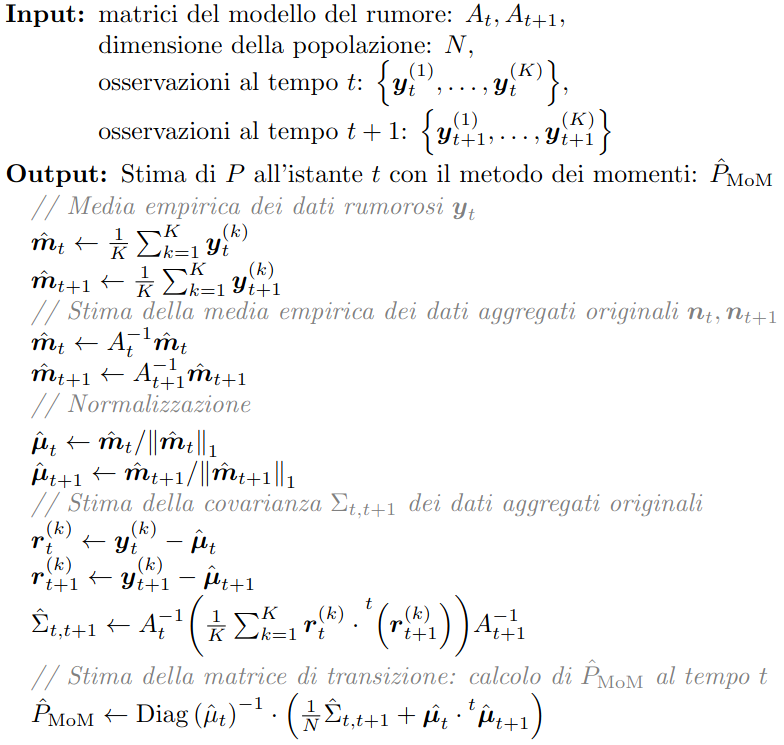
\includegraphics[width=0.65\textwidth]{Immagini/algorithm_nonstationary.png}
			%\caption{\emph{Algoritmo per il calcolo di $\hat{P}_{\textup{MoM}}$}}
		\end{figure}
		
	\end{frame}

	\begin{frame}[fragile]
		{Algoritmo per il calcolo di $\hat{P}_{\textup{MoM}}$ {\smaller (caso stazionario)}}
		Caso {\smaller (fortemente)} stazionario: $\pi_0=\pi$.

		\begin{figure}[ht]
			\centering
			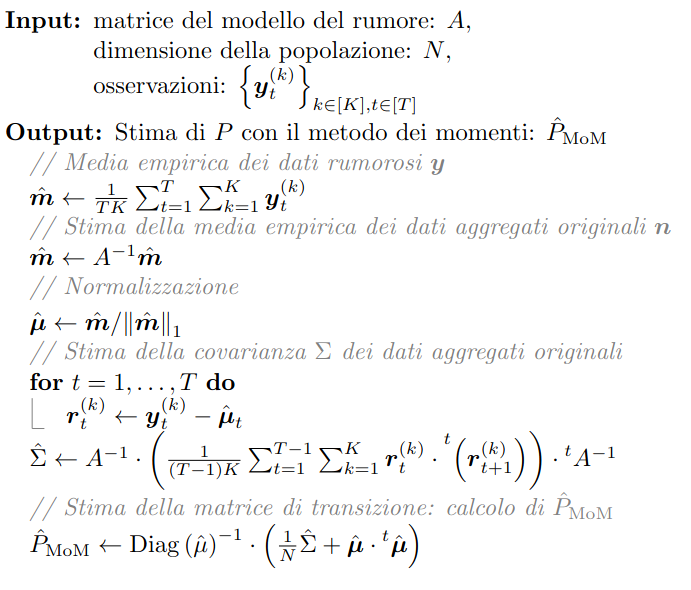
\includegraphics[width=0.65\textwidth]{Immagini/algorithm_stationary.png}
			%\caption{\emph{Algoritmo per il calcolo di $\hat{P}_{\textup{MoM}}$}}
		\end{figure}
		
	\end{frame}


	\subsection{Dimostrazione della consistenza di \texorpdfstring{$\hat{P}_{\textup{MoM}}$}{P_mom}}

	\begin{frame}
        {\hypertarget{frame:teorema_1_part1}{$\hat{P}_{\textup{MoM}}$ è consistente$\qquad 1/3$}}

        Supponiamo che:
        \begin{enumerate}
            \item $\pi_0=\pi$, ossia $\qty{x_t^{(m)}}_{t\in[T]}$ è \emph{fortemente} stazionario
            \item<2-> $\P{\vb*{y}}{\vb*{n}}$ rispetti le ipotesi della proposizione~\ref{prop:noise_model}
            \item<3-> $N\in\mathbb{N}, A\in\R{S}{S}$ siano noti {\smaller (e costanti: forte stazionarietà $\implies A_t=A\quad\forall\,t\in[T]$)}
        \end{enumerate}

        \begin{teorema}<4->\label{teor:consistenza_P_mom}
            Sia $\hat{P}_{T,K}$ lo stimatore restituito dall'algoritmo per il caso stazionario.

            Nelle ipotesi precedenti, $\hat{P}_{T,K}$ è consistente.%, ossia converge in probabilità 
            %a $P$ per $T\to\infty$ e/o $K\to\infty$.
        \end{teorema}
        \begin{block}<5->{Dimostrazione.}
            \begin{itemize}
                \item ${K\to\infty}$
                \begin{itemize}
                    \item<5-> Per la legge dei grandi numeri, $\lim_K\hat{\vb*{m}}_t=\mathbb{E}\qty[\vb*{y}_t]$ q.c.
                    \onslide<6->{Dunque 
                    $\lim_K\hat{\vb*{m}}=\lim_k\frac{1}{T}\sum_{t=1}^T\hat{\vb*{m}}_t=\mathbb{E}\qty[\vb*{y}_1]$ q.c.
                    (cfr. Appendice~\hyperlink{frame:teorema1_lim_mhat:appencide}{\faHandPointRight})}
                    \item<7-> Similmente si dimostra che $\lim_K\hat{\Sigma}_{t,t+1}=\Cov{\vb*{y}_1,\vb*{y}_2}$ q.c.
                    e dunque $\hat{\Sigma}=\frac{1}{T-1}\sum_{t=1}^{T-1}\hat{\Sigma}_{t,t+1}\overset{K\to\infty}{\longrightarrow}\Cov{\vb*{y}_1,\vb*{y}_2}$ q.c.
                    (cfr. Appendice~\hyperlink{frame:teorema1_lim_Sigmahat:appendice}{\faHandPointRight})
                \end{itemize}
                \onslide<8->{Ma allora $\hat{P}_{T,K}\overset{K\to\infty}{\longrightarrow}P$ in probabilità.}
            \end{itemize}
        \end{block}
    \end{frame}

    \begin{frame}
        {\hypertarget{frame:teorema_1_part2}{$\hat{P}_{\textup{MoM}}$ è consistente$\qquad 2/3$}}

        \begin{block}{}
            \begin{itemize}
                \item $T\to\infty$
                
                Possiamo supporre $K=1$. Dunque $\hat{\vb*{m}}_t=\vb*{y}_t$ e $\hat{\vb*{m}}=\frac{1}{T}\sum_{t=1}^{T}\vb*{y}_t$. \onslide<2->{Dobbiamo dimostrare che (in probabilità)
                \begin{gather*}
                    \hat{\vb*{m}}\xrightarrow{T\to\infty}\mathbb{E}\qty[\vb*{y}_1],\text{ e }\\
                    \hat{\Sigma}\coloneqq\frac{1}{T-1}\sum_{t=1}^{T-1}\qty(\vb*{y}_t-\hat{\vb*{m}})\cdot\transpose{\qty(\vb*{y}_{t+1}-\hat{\vb*{m}})}\xrightarrow{T\to\infty}\Cov{\vb*{y}_1,\vb*{y}_2}
                \end{gather*}}
                %in probabilità.
                \vspace{-\baselineskip}
                
                \hspace*{.05\linewidth}\begin{minipage}{.9\linewidth}
                    \begin{definizione*}<3->
                        $\qty{X_t}_{t\in[T]}$ {\smaller (fortemente stazionario)} è detto \emph{mean-ergodic} se $\frac{1}{T}\sum_{t=1}^TX_t$ converge in media seconda alla media della popolazione $\mathbb{E}\qty[X_t]$. 
                    \end{definizione*}
                    \begin{oss*}<4->
                        Convergenza in media seconda $\implies$ convergenza in probabilità.
                    \end{oss*}
                \end{minipage}
            \end{itemize}
        \end{block}

    \end{frame}

    \begin{frame}
        {\hypertarget{frame:teorema_1_part3}{$\hat{P}_{\textup{MoM}}$ è consistente$\qquad 3/3$}}

        \begin{block}{}
            $\hat{\vb*{y}}_t$ 
            mean-ergodic vuol dire che $\frac{1}{T}\sum_{t=1}^T\vb*{y}_t\xrightarrow{T\to\infty}\mathbb{E}\qty[\vb*{y}_1]$.
            \onslide<2->{Similmente, $\hat{\Sigma}\xrightarrow{T\to\infty}\Cov{\vb*{y}_1,\vb*{y}_2}$ se il processo $\qty{\vb*{Z}_t}_{t\in[T-1]}$, $\vb*{Z}_t\coloneqq\vb*{y}_t\cdot\transpose{\vb*{y}_{t+1}}$, è mean-ergodic.}

            \onslide<3->{Per dimostrarlo, è sufficiente dimostrare che $\qty{\vb*{Z}_t(i,j)}_{t\in[T-1]}$ è 
            mean-ergodic $\quad$ ({\smaller $\vb*{Z}_t(i,j)=\vb*{y}_{t}(i)\vb*{y}_{t+1}(j)$}).}
            
            \hspace{.05\linewidth}\begin{minipage}{.9\linewidth}
                \begin{block}<4->{Proposizione {\smaller~\cite[Theorem 12.2 (p.~528)]{book:Papoulis}}}
                    Sia $\qty{X_t}_{t\in[T]}$ stazionario e sia $\gamma_X(\tau)\coloneqq\Cov{X_{t+\tau},X_t}$ la sua funzione di autocovarianza. Se $\lim_{\tau\to\infty}\gamma_X(\tau)=0$ allora $\qty{X_t}_{t\in[T]}$ è mean-ergodic. 
                \end{block}                
            \end{minipage}
            \medskip
            
            \begin{enumerate}
                \item<5-> Consideriamo i processi $\qty{\vb*{n}_t}_{t\in[T]}$ e $\qty{z_t(i,j)}_{t\in[T-1]}$, $z_t(i,j)\coloneqq\vb*{n}_t(i)\vb*{n}_{t+1}(j)$ 
                \item<6-> Si dimostra che $\gamma_{\vb*{n}}(\tau)\xrightarrow{\tau\to\infty}0$ (cfr. Appendice~\hyperlink{frame:teorema1_lim_gamma_n:appendice}{\faHandPointRight}) e che $\gamma_z(i,j)\xrightarrow{\tau\to\infty}0$
                \item<7-> Si dimostra che $\qty{z_t(i,j)}_{t\in[T-1]}$ mean-ergodic $\implies\qty{\vb*{Z}_t(i,j)}_{t\in[T-1]}$ mean-ergodic, e che $\qty{\vb*{n}_t}_{t\in[T]}$ mean-ergodic $\implies\qty{\vb*{y}_t}_{t\in[T-1]}$ mean-ergodic.
            \end{enumerate}
            \hfill$\square$
        \end{block}
        
    \end{frame}












	

    
\section{Ringraziamenti e bibliografia}
    \begin{frame}
        \begin{center}
            \Huge{Grazie per l'attenzione!}
        \end{center}
    \end{frame}

	\begin{frame}{\refname}
		\begin{thebibliography}{9}
			\bibitem{article:main} Garrett Bernstein, Daniel Sheldon
			\newblock Consistently Estimating Markov Chains with Noisy Aggregate Data
			\newblock Proceedings of the 19th International Conference on Artificial Intelligence and Statistics, \emph{PMLR}, vol. 51, pp. 1142-1150, PMLR (2016) 09-11 May

			\bibitem{book:Norris} J. R. Norris
			\newblock Markov Chains
			\newblock Cambridge University Press, 1997

			\bibitem{book:Berger_Casella} R. L. Berger, G. Casella
			\newblock Statistical Inference (2nd ed.)
			\newblock Chapman and Hall/CRC, 2024

			\bibitem{book:Papoulis} A. Papoulis, S. U. Pillai
			\newblock Probability, Random Variables and Stochastic Processes (4th ed.)
			\newblock McGraw-Hill, 2002
		\end{thebibliography}
	\end{frame}

% ----------------------------------APPENDICE----------------------------------

\section*{Appendice}
	\begin{frame}
		\begin{center}
			\Huge{\textbf{Appendice}}
		\end{center}
	\end{frame}

	\begin{frame}
		{\hypertarget{frame:catena_ergodica:appendice}{Catene di Markov ergodiche}}
		\begin{definizione*}
			Ricordiamo che una catena di Markov è detta \alert{ergodica} se è
			irriducibile, positiva ricorrente e aperiodica.
		\end{definizione*}
		\onslide<2->{Una catena ergodica {\smaller (in quanto irriducibile e positiva 
		ricorrente)} ha una distribuzione invariante $\pi$. Inoltre:}
		\begin{itemize}
			\item<2-> $\pi$ è unica
			\item<3-> $\pi_i=1/\,\mathbb{E}_i\qty[T_i]$ 
			{\smaller (ovvero 1/tempo atteso di ritorno)}, dove 
			$T_i\coloneqq\inf_{n\ge 1}\qty{X_n=i}$ {\smaller (istante di primo passaggio)},
			e in particolare $\pi_i>0$			
		\end{itemize}
		\begin{oss*}<4->
			Per una catena finita e irriducibile {\smaller (dunque positiva ricorrente)},
			le due condizioni precedenti si possono ricavare dal teorema di Perron-Frobenius.
		\end{oss*}

		\onslide<5->{Il \emph{teorema di convergenza all'equilibrio} dice che per una 
		catena ergodica vale $\lim_{n\to\infty}\P{x_n=i}=\pi_i$. 
		In particolare $P_{i,j}\overset{n}{\longrightarrow}\pi_j\quad\forall\,i,j\in[S]$.}

		\blankfootnote{\textbf{Indietro:}~\hyperlink{frame:intro}{\faHandPointLeft}}
	\end{frame}

	\begin{frame}
		{\hypertarget{frame:dettagli_nt:appendice}{Dettagli sulla legge di $\vb*{n}_t$}}		
		$\R{S}\ni\vb*{n}_t$, e $\vb*{n}_t(i)=\sum_{m=1}^N\indicator$.
		\smallskip

		\onslide<2->{Possiamo interpretare $\vb*{n}_t$ come la somma di $N$ v.a. i.i.d.
		$V_t^{(1)},\dots,V_t^{(N)}$, ciascuna delle quali codifica lo stato 
		dell'individuo $m\in[N]$ corrispondente, al tempo $t\in[T]$.}

		\onslide<3->{$V_t^{(m)}$ rappresenta il risultato di una "prova" con $S$ 
		possibili \emph{outcomes}. L'outcome $i\in [S]$ è rappresentato dal versore 
		canonico $e_i\in\R{S}$.} 
		\onslide<4->{Si ha: 
		\[
			\P{V_t^{(m)}=e_i}=\P{x_t^{(m)}=i}=\vb*{\mu}_t(i)
		\]
		dunque $V_t^{(m)}$ è \emph{categorica} di parametro $\vb*{\mu}_t$, 
		$\forall\,m\in[N]$.} 
		\onslide<5->{Di conseguenza $\vb*{n}_t$ è multinomiale di 
		parametri $N,\vb*{\mu}_t$.}

		%\textcolor{red}{Disegno}
		\onslide<6->{\begin{figure}[ht]
			\centering
			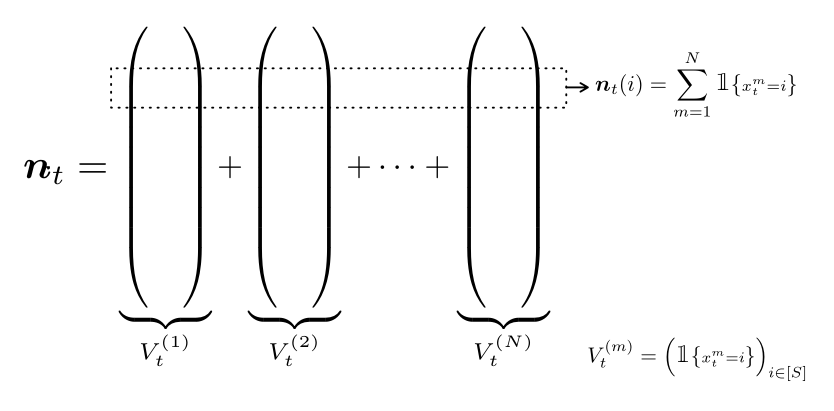
\includegraphics[width=0.5\textwidth]{Immagini/Disegno.png}
			%\caption{\emph{Algoritmo per il calcolo di $\hat{P}_{\textup{MoM}}$}}
		\end{figure}}
		
		\blankfootnote{\textbf{Indietro:}~\hyperlink{frame:dettagli_nt}{\faHandPointLeft}}
	\end{frame}

	\begin{frame}
		{\hypertarget{frame:dettagli_val_atteso_condiz_nt:appendice}{Calcolo di $\mathbb{E}\qty[\vb*{n}_t\mid\vb*{n}_{t-1}]$}}

		Sia $T_{i,j}^{(t-1)}$ la v.a. che conta il numero di individui che, all'istante $t-1\in[T]$,
		si spostano dallo stato $i\in[S]$ a $j\in[S]$. Allora $\vb*{n}_t(j)=\sum_{i=1}^S T_{i,j}^{(t-1)}$.
		\smallskip

		\onslide<2->{Conoscendo $\vb*{n}_{t-1}(i)$, $T_{i,j}^{(t-1)}$ è 
		binomiale di parametri $\vb*{n}_{t-1}(i)$ e $P_{i,j}$:
		%$\P{T_{i,j}^{(t-1)}}{\vb*{n}_{t-1}}=\mathcal{B}\qty(\vb*{n}_t(i),(P_{i,j},1-P_{i,j});2)$
		\[
			\P{T_{i,j}^{(t-1)}=\alpha}{\vb*{n}_{t-1}}=\smqty(\vb*{n}_{t-1}(i)\\ \alpha)\cdot P_{i,j}^{\alpha}\cdot(1-P_{i,j})^{1-\alpha}
		\]}
		%\vspace*{-0.5\baselineskip}

		\onslide<3->{Ne segue che 
		\vspace*{-0.5\baselineskip}
		\begin{align*}
			\mathbb{E}\qty[\vb*{n}_t(j)\mid\vb*{n}_{t-1}]&=\sum_{i=1}^S \mathbb{E}\qty[T_{i,j}^{(t-1)}\mid\vb*{n}_{t-1}]=\sum_{i=1}^{S}\mathbb{E}\qty[T_{i,j}^{(t-1)}\mid\vb*{n}_{t-1}(i)]\\
			&=\sum_{i=1}^{S}\vb*{n}_{t-1}(i)P_{i,j}=\qty(\transpose{\vb*{n}_{t-1}}P)_j
		\end{align*}
		Ovvero $\mathbb{E}\qty[\vb*{n}_t\mid\vb*{n}_{t-1}]=\transpose{\vb*{n}_{t-1}}P$.}


		\blankfootnote{\textbf{Indietro:}~\hyperlink{frame:CLS}{\faHandPointLeft}}
	\end{frame}

	\begin{frame}
		{\hypertarget{frame:dim_prop_1:appendice}{Dimostrazione della Proposizione~\ref{prop:formule_momenti}$\qquad$ 1/4}}
		\begin{block}{Dimostrazione.}
			$\vb*{n}_t$ è multinomiale di parametri $N$ e $\vb*{\mu}_t$, 
			$\vb*{n}_t=\sum_{m=1}^{N}V_t^{(m)}$, con $V_t^{(m)}$ categorica di parametro $\vb*{\mu}_t$,
			e $V_t^{(m)}\independent V_t^{(m')}\quad\forall m\ne m'$. Ometteremo l'apice quando sarà irrilevante.
			\begin{enumerate}
				\item\label{proof:prop_1:point_1} $\mathbb{E}\qty[\vb*{n}_t]=N\vb*{\mu}_t$ è un risultato noto sulle v.a. multinomiali. 
				Segue dal fatto che $\vb*{n}_t(i)$ è binomiale di parametri $N$ e $\vb*{\mu}_t(i)$. 
				\smallskip

				Comunque,
				$\mathbb{E}\qty[\vb*{n}_t]=\sum_{m=1}^{N}\mathbb{E}\qty[V_t^{(m)}]=N\,\mathbb{E}\qty[V_t]$, e si ha
				\vspace{-0.5\baselineskip}
				\begin{align*}
					\R{S}\ni\mathbb{E}\qty[V_t]&=\sum_{i=1}^{S}e_i\cdot\P{V_t=e_i}=\sum_{i=1}^{S}e_i\cdot\P{V_t(i)=1}\\
					& = \sum_{i=1}^{S}e_i\cdot\P{\indicator[t][{}][i]=1}=\sum_{i=1}^{S}e_i\cdot\vb*{\mu}_t(i)=\vb*{\mu}_t
				\end{align*}
				da cui segue che $\vb*{m}_t=\mathbb{E}\qty[\vb*{n}_t]=N\,\vb*{\mu}_t$.				
			\end{enumerate}
		\end{block}
	
		\blankfootnote{\textbf{Indietro:}~\hyperlink{frame:prop_1}{\faHandPointLeft}}
	\end{frame}

	\begin{frame}
		{Dimostrazione della Proposizione~\ref{prop:formule_momenti}$\qquad$ 2/4}
		
		\begin{block}{}
			\begin{enumerate}
				\setcounter{enumi}{1}
				\item Per indipendenza e per il punto~\eqref{proof:prop_1:point_1} si ha
				\vspace{-0.5\baselineskip}
				\begin{align*}
					\Sigma_t&=\Var{\vb*{n}_t}=\sum_{m=1}^{N}\Var{V_t^{(m)}}=N\cdot\Var{V_t}\\
					&=N\cdot(\mathbb{E}\qty[V_t\transpose{V_t}]-\mathbb{E}\qty[V_t]\cdot\mathbb{E}\qty[\transpose{V_t}])=N\cdot(\mathbb{E}\qty[V_t\transpose{V_t}]-\vb*{\mu}_t\transpose{\vb*{\mu}_t})
				\end{align*}
				Ora, $\R{S}{S}\ni\mathbb{E}\qty[V_t\transpose{V_t}]$ è t.c.
				\vspace{-0.5\baselineskip}
				\begin{align*}
					\mathbb{E}\qty[V_t\transpose{V_t}]_{i,j}&=\mathbb{E}\qty[V_t(i)\cdot V_t(j)]=\smashoperator[rl]{\sum_{\alpha,\beta=0}^{1}}\alpha\beta\cdot\P{V_t(i)=\alpha,V_t(j)=\beta}\\
					& = \P{V_t(i)=1,V_t(j)=1}=
					\begin{dcases*}
						0 & se $i\ne j$\\
						\vb*{\mu}_t(i) & se $i=j$
					\end{dcases*}
				%\intertext{$V_t\in\qty{e_1,\dots,e_S}$, quindi non può
				%assumere valore 1 su due componenti diverse. Ne segue che}
				%	&  \P{V_t(i)=1,V_t(j)=1}=
				%	\begin{dcases*}
				%		0 & se $i\ne j$\\
				%		\vb*{\mu}_t(i) & se $i=j$
				%	\end{dcases*}\\
				\end{align*}
				Infatti $V_t\in\qty{e_1,\dots,e_S}$, quindi non può
				assumere valore 1 su due componenti diverse.

				Dunque $\mathbb{E}\qty[V_t\transpose{V_t}]=\operatorname{Diag}\qty(\vb*{\mu}_t)$ 
				e si ha $\Sigma_t=N\cdot(\operatorname{Diag}\qty(\vb*{\mu}_t)-\vb*{\mu}_t\transpose{\vb*{\mu}_t})$
			\end{enumerate}
		\end{block}

		\blankfootnote{\textbf{Indietro:}~\hyperlink{frame:prop_1}{\faHandPointLeft}}
	\end{frame}

	\begin{frame}
		{Dimostrazione della Proposizione~\ref{prop:formule_momenti}$\qquad$ 3/4}
		
		\begin{block}{}
			\begin{enumerate}
				\setcounter{enumi}{2}
				\item Si ha 
				\vspace*{-\baselineskip}
				\begin{align*}
					\Sigma_{t,t+1}&=\Cov{\sum_{m=1}^N V_{t}^{(m)},\sum_{m'=1}^N V_{t+1}^{(m')}}=\smashoperator[lr]{\sum_{m,m'}}\Cov{V_t^{(m)},V_{t+1}^{(m')}}\\
					&=\sum_{m=m'}\Cov{V_t^{(m)},V_{t+1}^{(m)}}+\sum_{m\ne m'}\Cov{V_t^{(m)},V_{t+1}^{(m')}}=
				\intertext{per indipendenza si ha}
					&=\sum_{m=m'}\Cov{V_t^{(m)},V_{t+1}^{(m)}}+0=N\cdot\Cov{V_t,V_{t+1}} .
				\end{align*}
				Dunque $\Sigma_{t,t+1}=N\cdot\Cov{V_t,V_{t+1}}=N\cdot\qty(\mathbb{E}\qty[V_t\transpose{V_{t+1}}]-\vb*{\mu}_t\transpose{\vb*{\mu}_{t+1}}).$
				\smallskip

				Procedendo in maniera analoga al punto precedente si dimostra che 
				\vspace*{-0.25\baselineskip}
				\[
					\mathbb{E}\qty[V_t\transpose{V_{t+1}}]_{i,j}=\P{V_t(i)=1,V_{t+1}(j)=1}=\vb*{\mu}_{t,t+1}(i,j)
				\]
				%\vspace*{-0.5\baselineskip}
				da cui segue che $\Sigma_{,t+1}=N\cdot\qty(\vb*{\mu}_{t,t+1}-\vb*{\mu}_t\transpose{\vb*{\mu}_{t+1}}).$
			\end{enumerate}			
		\end{block}

		\blankfootnote{\textbf{Indietro:}~\hyperlink{frame:prop_1}{\faHandPointLeft}}
	\end{frame}

	\begin{frame}
		{Dimostrazione della Proposizione~\ref{prop:formule_momenti}$\qquad$ 4/4}

		\begin{block}{}
			\begin{enumerate}
				\setcounter{enumi}{3}
				\item Si ha che $\Lambda_{t}=\mathbb{E}\qty[\vb*{n}_t\transpose{\vb*{n}_t}]$ per definizione,
				ma 
				\begin{align*}
					\mathbb{E}\qty[\vb*{n}_t\transpose{\vb*{n}_t}]&=\Var{\vb*{n}_t}+\mathbb{E}\qty[\vb*{n}_t]\cdot\mathbb{E}\qty[\transpose{\vb*{n}_t}]\\
					&=\Sigma_t+N^2\cdot\vb*{\mu}_t\transpose{\vb*{\mu}_t}=N\cdot\qty(\operatorname{Diag}(\vb*{\mu}_t)+(N-1)\vb*{\mu}_t\transpose{\vb*{\mu}_t})
				\end{align*}
				\item Per definizione $\Lambda_{t,t+1}=\mathbb{E}\qty[\vb*{n}_t\transpose{\vb*{n}_{t+1}}]$, 
				quindi identicamente al punto precedente
				\begin{align*}
					\mathbb{E}\qty[\vb*{n}_t\transpose{\vb*{n}_{t+1}}]&=\Cov{\vb*{n}_t,\vb*{n}_{t+1}}+\mathbb{E}\qty[\vb*{n}_t]\cdot\mathbb{E}\qty[\transpose{\vb*{n}_{t+1}}]\\
					&=\Sigma_{t,t+1}+N^2\cdot\vb*{\mu}_t\transpose{\vb*{\mu}_{t,t+1}}\\
					&=N\cdot\qty(\vb*{\mu}_{t,t+1}+(N-1)\vb*{\mu}_t\transpose{\vb*{\mu}_{t+1}})
				\end{align*}
			\end{enumerate}%\qedsymbol
			ossia la tesi.\hfill\qedsymbol
		\end{block}

		\blankfootnote{\textbf{Indietro:}~\hyperlink{frame:prop_1}{\faHandPointLeft}}		
	\end{frame}

	\begin{frame}
		{\hypertarget{frame:dim_prop_2:appendice}{Dimostrazione $P=\Lambda_t^{-1}\Lambda_{t,t+1}\qquad 1/2$}}
	
		\begin{block}{Dimostrazione.}
			$\Lambda_t=N\cdot\qty(\operatorname{Diag}\qty(\vb*{\mu}_t)+(N-1)\vb*{\mu}_t\transpose{\vb*{\mu}_{t+1}})$
			è somma di una matrice invertibile e di una matrice di rango 1, dunque è invertibile.

			Esiste un'espressione esplicita per $\Lambda_t$ (formula di Sherman-Morrison): 
			denotando $D\equiv\operatorname{Diag}\qty(\vb*{\mu}_t)$ e con $\vb*{e}$ il 
			vettore con tutte le entrate uguali a $1$,
			\begin{align*}
				\Lambda_t^{-1}&=\frac{1}{N}\qty(D+(N-1)\vb*{\mu}_t\transpose{\vb*{\mu}_t})^{-1}\\
				&=\frac{1}{N}\qty(D^{-1}-\frac{(N-1)D^{-1}\vb*{\mu}_t\transpose{\vb*{\mu}_t}D^{-1}}{1+(N-1)\transpose{\vb*{\mu}_t}D^{-1}\vb*{\mu}_t})\\
				&=\frac{1}{N}\qty(D^{-1}-\frac{N-1}{N}\vb*{e}\transpose{\vb*{e}})
			\end{align*}
			Infatti $D^{-1}\vb*{\mu}_t=\vb*{e}$, e poiché 
			$\vb*{\mu}_t$ è un vettore stocastico $\langle\vb*{e},\vb*{\mu}_t\rangle=1$.
		\end{block}

		\blankfootnote{\textbf{Indietro:}~\hyperlink{frame:CLS_as_moment}{\faHandPointLeft}}
	\end{frame}

	\begin{frame}
		{Dimostrazione $P=\Lambda_t^{-1}\Lambda_{t,t+1}\qquad 2/2$}
		
			\begin{block}{}
				Dimostriamo dunque che $\Lambda_tP=\Lambda_{t,t+1}$:
				\begin{align*}
					\Lambda_tP&=N\qty(D+(N-1)\vb*{\mu}_t\transpose{\vb*{\mu}_t})P\\
					&=N\qty(DD^{-1}\vb*{\mu}_{t,t+1}+(N-1)\vb*{\mu}_t\transpose{\vb*{\mu}_t}P)\\
					&=N\qty(\vb*{\mu}_{t,t+1}+(N-1)\vb*{\mu}_t\transpose{\vb*{\mu}_{t+1}})=\Lambda_{t,t+1}
				\end{align*}
				ossia la tesi.\hfill\qedsymbol
			\end{block}

		\blankfootnote{\textbf{Indietro:}~\hyperlink{frame:CLS_as_moment}{\faHandPointLeft}}
	\end{frame}


	\begin{frame}
		{\hypertarget{frame:dim_prop_noise_model:appendice}{Dimostrazione della proposizione~\ref{prop:noise_model}}}

		\begin{proof}
			\begin{enumerate}
				\item $\mathbb{E}\qty[\vb*{y}_t]=\mathbb{E}\qty[\,\mathbb{E}\qty[\vb*{y}_t\mid\vb*{n}_t]\,]=\mathbb{E}\qty[A_t\vb*{n}_t]=A_t\cdot\mathbb{E}\qty[\vb*{n}_t]$
				\item Si ha 
				\begin{align*}
					\mathbb{E}\qty[\vb*{y}_s\transpose{\vb*{y}_t}]&=\mathbb{E}\qty[\,\mathbb{E}\qty[\vb*{y}_s\transpose{\vb*{y}_t}\mid \vb*{n}_s,\vb*{n}_t]\,]
					=\mathbb{E}\qty[\,\mathbb{E}\qty[\vb*{y}_s\mid \vb*{n}_s,\vb*{n}_t]\cdot\mathbb{E}\qty[\transpose{\vb*{y}_t}\mid\vb*{n}_s,\vb*{n}_t]\,]\\
					&=\mathbb{E}\qty[\,\mathbb{E}\qty[\vb*{y}_s\mid \vb*{n}_s]\cdot\mathbb{E}\qty[\transpose{\vb*{y}_t}\mid\vb*{n}_t]\,]
					=\mathbb{E}\qty[\,A_s\cdot\vb*{n}_s\transpose{\vb*{n}_t}\cdot\transpose{A_t}\,]\\
					&=A_s\cdot\mathbb{E}\qty[\vb*{n}_s\transpose{\vb*{n}_t}]\cdot\transpose{A_t}
				\end{align*}
				\item Si ha, per i due punti precedenti,
				\begin{align*}
					\Cov{\vb*{y}_s,\vb*{y}_t}&=\mathbb{E}\qty[\vb*{y}_s\transpose{\vb*{y}_t}]-\mathbb{E}\qty[\vb*{y}_s]\cdot\mathbb{E}\qty[\transpose{\vb*{y}_t}]\\
					&=\mathbb{E}\qty[\vb*{y}_s\transpose{\vb*{y}_t}]-A_s\cdot\mathbb{E}\qty[\vb*{y}_t]\mathbb{E}\qty[\transpose{\vb*{y}_t}]\cdot\transpose{A_t}\\
					&=A_s\cdot\qty(\mathbb{E}\qty[\vb*{n}_s\transpose{\vb*{n}_t}]-\mathbb{E}\qty[\vb*{y}_t]\mathbb{E}\qty[\transpose{\vb*{y}_t}])\cdot\transpose{A_t}
				\end{align*}
			\end{enumerate}
			Dall'invertibilità di $A_s$ e $A_t$ segue la tesi.
		\end{proof}

		\blankfootnote{\textbf{Indietro:}~\hyperlink{frame:prop_noise_model}{\faHandPointLeft}}
	\end{frame}

	\begin{frame}
        {Consistenza di \texorpdfstring{$\hat{P}_{T,K}$}{P_T,K} per \texorpdfstring{$K\to\infty$}{K tendente a infinito}$\qquad 1/2$}
        {\hypertarget{frame:teorema1_lim_mhat:appencide}{Dettagli sul calcolo di \texorpdfstring{$\lim_K\hat{\vb*{m}}$}{un limite}}}

        %\begin{block}{}
        Nel calcolo di $\lim_K\hat{\vb*{m}}$ si fa uso dell'ipotesi di stazionarietà:
        \begin{align*}
            \lim_K\hat{\vb*{m}}&=\lim_K\frac{1}{T}\sum_{t=1}^T\hat{\vb*{m}}_t=\frac{1}{T}\sum_{t=1}\
            \lim_K\hat{\vb*{m}}_t=\frac{1}{T}\sum_{t=1}^T\mathbb{E}\qty[\vb*{y}_t]\
            =\frac{1}{T}\sum_{t=1}^T A_t\mathbb{E}\qty[\vb*{n}_t]\\
        \intertext{Per ipotesi $A_t=A\quad\forall\,t\in[T]$. Dunque}
            &=\frac{1}{T}\cdot A\cdot\sum_{t=1}^T\mathbb{E}\qty[\vb*{n}_t]=\frac{1}{T}\cdot A\cdot T\cdot\mathbb{E}\qty[\vb*{n}_1]=A\cdot\mathbb{E}\qty[\vb*{n}_1]=\mathbb{E}\qty[\vb*{y}_1]
        %\intertext{Ma per stazionarietà $\mathbb{E}\qty[\vb*{n}_t]=\mathbb{E}\qty[\vb*{n}_1]\quad\forall\,t\in[T]$. Dunque}
        \end{align*}
        poiché per stazionarietà $\mathbb{E}\qty[\vb*{n}_t]=\mathbb{E}\qty[\vb*{n}_1]\quad\forall\,t\in[T]$.
        %\end{block}

        \blankfootnote{\textbf{Indietro:}~\hyperlink{frame:teorema_1_part1}{\faHandPointLeft}}
    \end{frame}

    \begin{frame}
        {Consistenza di \texorpdfstring{$\hat{P}_{T,K}$}{P_T,K} per \texorpdfstring{$K\to\infty$}{K tendente a infinito}$\qquad 2/2$}
        {\hypertarget{frame:teorema1_lim_Sigmahat:appendice}{Dettagli sul calcolo di \texorpdfstring{$\lim_k\hat{\Sigma}_{t,t+1}$}{un altro limite}}}

        %\begin{block}{}
        Consideriamo 
        \[
            \hat{\Sigma}_{t,t+1}=\frac{1}{K}\sum_{k=1}^{K}\qty(\vb*{y}_t^{(k)}-\hat{\vb*{m}}_t)\cdot\transpose{\qty(\vb*{y}_{t+1}^{(k)}-\hat{\vb*{m}}_{t+1})}=\frac{1}{K}\sum_{k=1}^{K}\qty(\vb*{y}_t^{(k)}\cdot\transpose{\vb*{y}}_{t+1}^{(k)})-\hat{\vb*{m}}_t\cdot\transpose{\hat{\vb*{m}}_{t+1}}
        \]
        Per la legge dei grandi numeri $\hat{\vb*{m}}_t\xrightarrow{K\to\infty}\mathbb{E}\qty[\vb*{y}_t]$ q.c.,
        e $\frac{1}{K}\sum_{k=1}^K\vb*{y}_t^{(k)}\cdot\transpose{\vb*{y}}_{t+1}^{(k)}\xrightarrow{K\to\infty}\mathbb{E}\qty[\vb*{y}_t\cdot\transpose{\vb*{y}_{t+1}}]$ q.c.
        \medskip

        Dunque {\smaller (due applicazioni del teorema di Slusky~\cite[Theorem~5.5.17]{book:Berger_Casella})} $\hat{\vb*{m}}_t\cdot\transpose{\hat{\vb*{m}}}_{t+1}\xrightarrow{K\to\infty}\mathbb{E}\qty[\vb*{y}_t]\cdot\mathbb{E}\qty[\transpose{\vb*{y}}_{t+1}]$ in legge. Ma il valore atteso è una costante, quindi la convergenza è in probabilità. 

        Poiché la convergenza quasi certa implica quella in probabilità, si ha che 
        \[
            \hat{\Sigma}_{t,t+1}\xrightarrow{K\to\infty}\mathbb{E}\qty[\vb*{y}_t\cdot\transpose{\vb*{y}_{t+1}}]-\mathbb{E}\qty[\vb*{y}_t]\cdot\mathbb{E}\qty[\transpose{\vb*{y}}_{t+1}]=\Cov{\vb*{y}_1,\vb*{y}_2}
        \]
        in quanto per stazionarietà $\Cov{\vb*{y}_t,\vb*{y}_{t+1}}=\Cov{\vb*{y}_1,\vb*{y}_2}\quad\forall\,t\in[T]$.
        %\end{block}

        \blankfootnote{\textbf{Indietro:}~\hyperlink{frame:teorema_1_part1}{\faHandPointLeft}}
    \end{frame}

    \begin{frame}
        {Consistenza di \texorpdfstring{$\hat{P}_{T,K}$}{P_T,K} per \texorpdfstring{$T\to\infty$}{K tendente a infinito}}
        {\hypertarget{frame:teorema1_lim_gamma_n:appendice}{Dimostrazione di $\lim_{\tau}\gamma_{\vb*{n}}(\tau)=0$}}

        %\begin{block}{}
        Consideriamo $\qty(\gamma_{\vb*{n}}(\tau))_i=\Cov{\vb*{n}_t(i),\vb*{n}_{t+\tau}(i)}\equiv\gamma_{\vb*{n}(i)}(\tau)$.
        \begin{align*}
            \gamma_{\vb*{n}(i)}(\tau)&=\operatorname{Cov}\bigg(\sum_{m=1}^N\indicator,\sum_{m'=1}^N\indicator[t+\tau][m'][i]\bigg)\\
            %\begin{aligned}[t]
            &=\sum_{m=m'}\Cov{\indicator,\indicator[t+\tau][m][i]}+\sum_{m\ne m'}\cancel{\Cov{\indicator,\indicator[t+\tau][m'][i]}}\\
            %\end{aligned}\\
            &=N\Big(\mathbb{E}\qty[\indicator\indicator[t+\tau]]-\mathbb{E}\qty[\indicator]\mathbb{E}\qty[\indicator[t+\tau]]\Big)\\
            &=N\Big(\P{x_{t+\tau}^{m}=i,x_t^{m}=i}-\P{x_t^m=i}\P{x_{t+\tau}^m=i}\Big)\\
            &=N\Big(\P{x_{t+\tau}^m=i}{x_t^{m}=i}\P{x_t^m=i}-\vb*{\mu}_t(i)\cdot\vb*{\mu}_{t+\tau}(i)\Big)\\
            &=N\vb*{\mu}_t(i)\cdot\Big(P^{\tau}_{i,i}-\vb*{\mu}_{t+\tau}(i)\Big)\xrightarrow{\tau\to\infty}0
        \end{align*}
        in quanto per l'ergodicità $\lim_{\tau}\vb*{\mu}_{t+\tau}=\pi$ e $\lim_{\tau}P_{i,j}^{\tau}=\pi_j\quad\forall\,i,j\in[S]$.%\hfill$\square$
        %\end{block}


        \blankfootnote{\textbf{Indietro:}~\hyperlink{frame:teorema_1_part3}{\faHandPointLeft}}
    \end{frame}



\end{document}

